\documentclass[]{article}
\usepackage{graphicx}
\usepackage{subfig}
\usepackage{amsmath}
\usepackage{amsfonts}
\usepackage[margin=1in]{geometry}

\begin{document}



\begin{center}
\begin{figure}[!ht]
\centering
\subfloat[Accuracy]{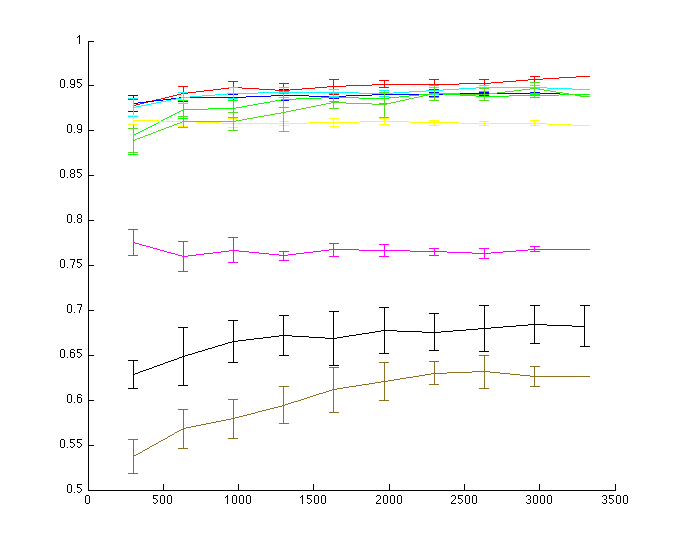
\includegraphics[width=.7\textwidth]{../images/c3.png}}
\subfloat[Legend]{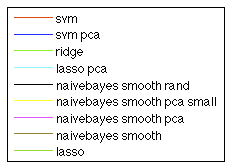
\includegraphics[width=.3\textwidth]{../images/legend.png}}
\caption{Accuracy vs Size of subsampled training data used.}
\label{fig:largecompare}
\end{figure}
\end{center}

\begin{center}
\begin{figure}[!ht]
\centering
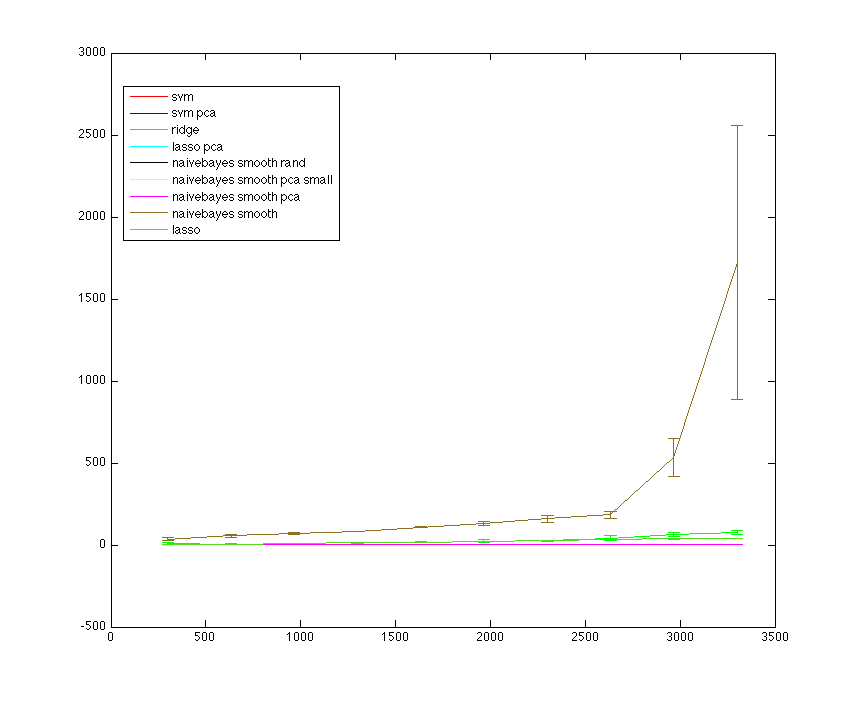
\includegraphics[width=.7\textwidth]{../images/c3time.png}
\caption{Time vs Size of subsampled training data used.}
\label{fig:largecompare}
\end{figure}
\end{center}



\begin{tabular}{lcc}
\hline
& Mean & STD \\
\hline
svm & .9600 & 2.3406e-16\\
svm pca & 0.9400 & 2.3406e-16\\
ridge & 0.9400 & 2.3406e-16\\
lasso pca & 0.9460 & 0 \\
naivebayes smooth rand & 0.6826 & 0.0226\\
naivebayes smooth pca small & 0.9060 & 0\\
naivebayes smooth pca & 0.7680 & 1.1703e-16\\
lasso & 0.9380 & 0\\
naivebayes smooth & 0.6260 & 1.1703e-16
\end{tabular}
\begin{center}
\begin{figure}[!ht]
\centering
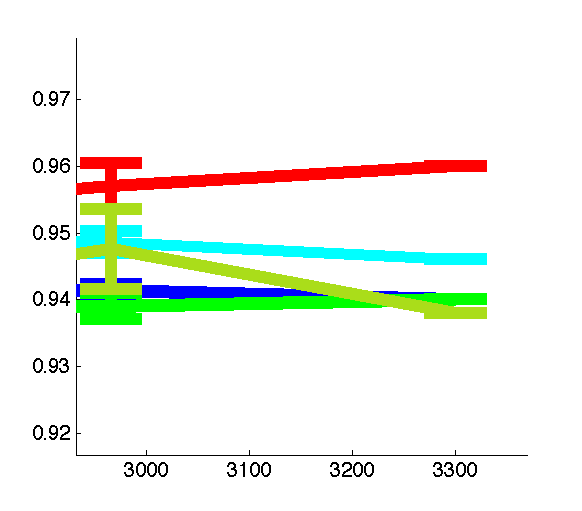
\includegraphics[width=.7\textwidth]{../images/c3zoombig.png}
\caption{Accuracy vs Size of subsampled training data used.}
\label{fig:largecomparekleg}
\end{figure}
\end{center}
\end{document}
